\documentclass[12pt]{extarticle}
\usepackage{tempora}
\usepackage[T1, T2A]{fontenc}
\usepackage[utf8]{inputenc}
\usepackage[english, ukrainian]{babel}
\usepackage{geometry}
\usepackage{graphicx}
\usepackage{multirow}
\usepackage{multicol}
\usepackage{float}
\graphicspath{{/home/artem/Pictures}}
\geometry
{
    a4paper,
    left=30mm,
    top=15mm,
    right=20mm,
    bottom=15mm,
}

\begin{document}
\begin{titlepage}
    \begin{center}
        \textbf{\normalsize{\MakeUppercase{
            Міністерство Освіти і науки України
            Національний університет "Львівська політехніка"
        }}}

        \begin{flushright}
        \textbf{ІКНІ}\\
        Кафедра \textbf{ПЗ}
        \end{flushright}
        \vspace{15mm}

        \includegraphics[width=0.4\textwidth]{lpnu_logo.png}

        \vspace*{\fill}

        \textbf{\normalsize{\MakeUppercase{Звіт}}}
            
        До лабораторної роботи №3

        \textbf{на тему:} “СИНТЕЗ ТА МОДЕЛЮВАННЯ ОСНОВНИХ ТИПІВ РЕГІСТРІВ ТА
        ЛІЧИЛЬНИКІВ В СИСТЕМІ PROTEUS”

        \textbf{з дисципліни:} “Архітектура комп’ютера”
            
        \vspace*{\fill}

        \begin{flushright}

            \textbf{Лектор:}\\
            доцент кафедри ПЗ\\
            Крук О.Г.\\
            \vspace{12pt}

            \textbf{Виконав:}\\
            студент групи ПЗ-24\\
            Губик А. С.\\
            \vspace{12pt}

            \textbf{Прийняв:}\\
            доцент кафедри ПЗ\\
            Задорожний І. М.\\
        \vspace{12pt}
        \end{flushright}

        Львів -- 2023
            
            
    \end{center}
\end{titlepage}

\textbf{Тема роботи:} синтез та моделювання оснивних 
типів регістрів та лічильників в системі Proteus

\vspace{12pt}

\textbf{Мета роботи:} поглибити знання про будову та функціонування основних типів
регістрів та лічильників; синтезувати їх схеми та виконати
моделювання в системі програм Proteus; дослідити на основі
отриманих часових діаграм їх роботу.

\subsection*{Індивідуальне завдання}
\begin{center}
    \begin{tabular}{| c | c | c | c | c | c |}
        \hline
        Варіант & n & $a_1 ... a_n$ & $M_a$ & $M_c$ & $f_0$, КГц\\
        \hline
           3  & 5 & 28, 17, 63, 42, 88 & 26 &   22  &    190\\
        \hline
   
    \end{tabular}
\end{center}

\subsection*{Теоретичні відомості}
Регістр - це типовий функціональний вузол комп’ютера, призначений для
приймання, тимчасового зберігання, перетворення і видавання n-розрядного
двійкового слова. Регістр містить регулярний набір однотипових тригерів, в
кожному з яких зберігається значення одного двійкового розряду машинного
слова. Найчастіше використовують тригери типів D, RS та JK.
Регістри, призначені тільки для приймання (записування), зберігання і
видавання інформації, називаються елементарними або регістрами пам’яті, або ж
фіксаторами. Регістри пам’яті - це пристрої з паралельним записуванням
та зчитуванням інформації, яка подана в паралельному коді. Записана у тригери
інформація може зчитуватись у прямому коді, інверсному або одночасно в прямому
та інверсному кодах.
Вони можуть бути синхронізовані рівнем або фронтом тактового сигналу
залежно від типу застосовуваних тригерів. Елементарні регістри будують на
одноступеневих тригерах. Логічна функція регістра позначається буквами RG
Лічильник - це типовий функціональний вузол комп'ютера, призначений для
лiчби та фіксації вхідних імпульсів. Лічильник складається із послідовно зв’язаних
Т-тригерів, які утворюють пам’ять iз заданим числом сталих станів 
(register).
\subsection*{Хід роботи}
\paragraph{1.}x

\vspace{12pt}
\begin{figure}[H]
    \centering
    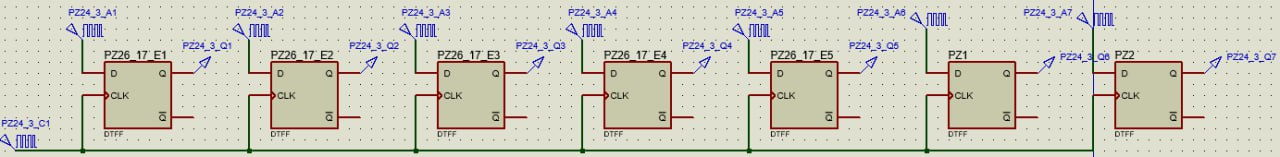
\includegraphics[width=0.90\textwidth]{register.jpg}
    \caption{Регістр}
\end{figure}
\begin{figure}[H]
    \centering
    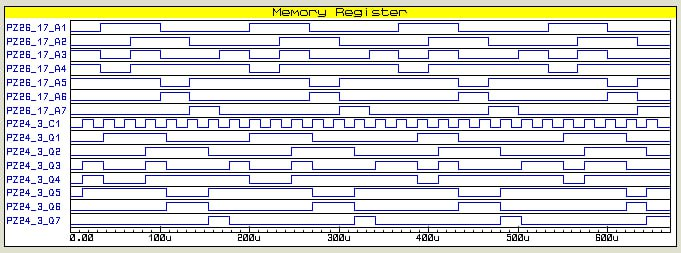
\includegraphics[width=0.90\textwidth]{register_graph.jpg}
    \caption{Графік}
\end{figure}

\paragraph{2.}x
\begin{figure}[H]
    \centering
    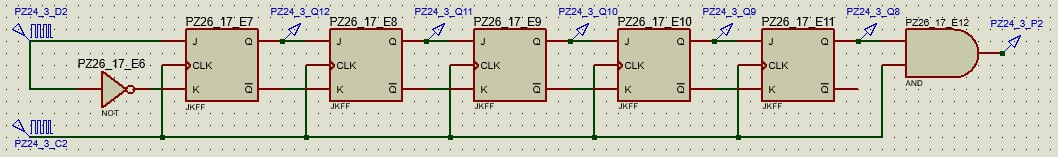
\includegraphics[width=0.90\textwidth]{shift.jpg}
    \caption{Регістр зсуву}
\end{figure}
\begin{figure}[H]
    \centering
    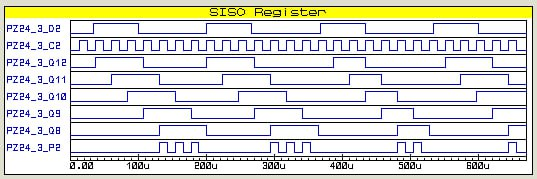
\includegraphics[width=0.90\textwidth]{shift_graph.jpg}
    \caption{Графік}
\end{figure}

\vspace{12pt}

\paragraph{3.}x

\begin{figure}[H]
    \centering
    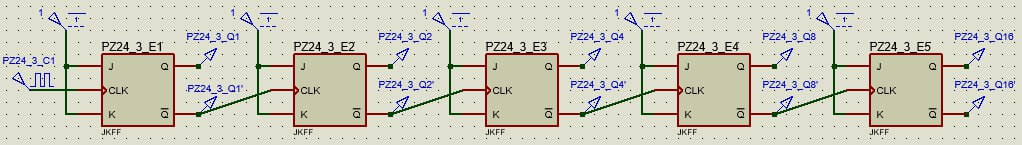
\includegraphics[width=0.90\textwidth]{async_counter.jpg}
    \caption{Асинхронний лічильник}
\end{figure}
\begin{figure}[H]
    \centering
    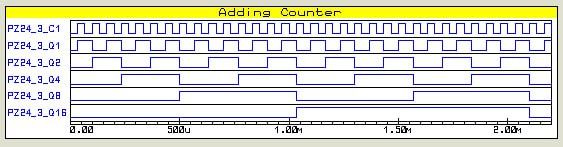
\includegraphics[width=0.90\textwidth]{async_counter_graph_add.jpg}
    \caption{Графік прямих виходів}
\end{figure}
\begin{figure}[H]
    \centering
    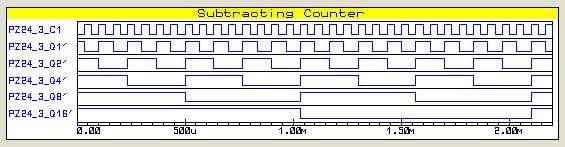
\includegraphics[width=0.90\textwidth]{async_counter_graph_sub.jpg}
    \caption{Графік непрямих виходів}
\end{figure}
\paragraph{4.}x
\begin{figure}[H]
    \centering
    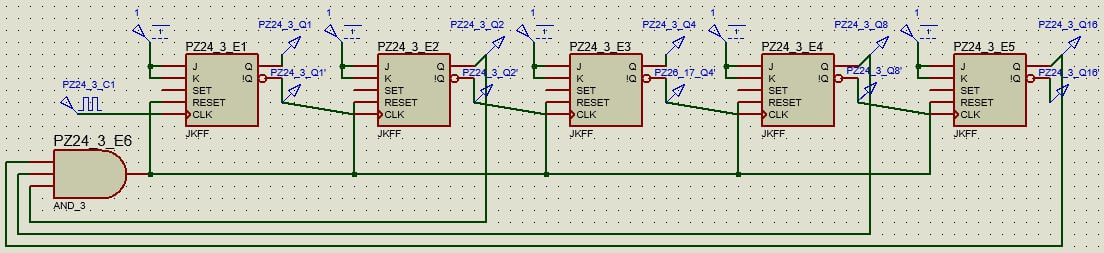
\includegraphics[width=0.90\textwidth]{async_mod_counter.jpg}
    \caption{Синхронний лічильник по модулю 26}
\end{figure}
\begin{figure}[H]
    \centering
    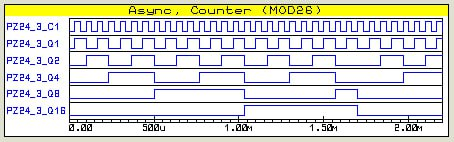
\includegraphics[width=0.90\textwidth]{async_mod_counter_graph.jpg}
    \caption{Графік}
\end{figure}
\paragraph{5.}x
\begin{figure}[H]
    \centering
    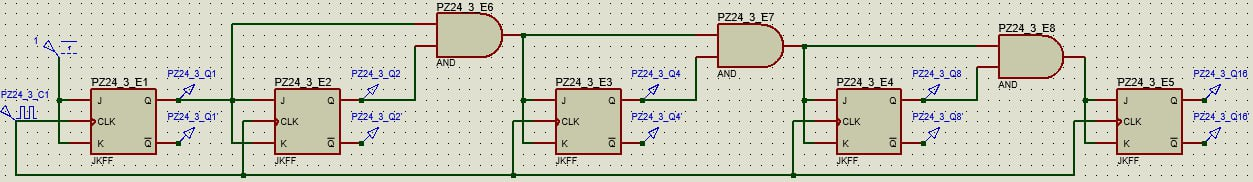
\includegraphics[width=0.90\textwidth]{sync_counter.jpg}
    \caption{Синхронний лічильник}
\end{figure}
\begin{figure}[H]
    \centering
    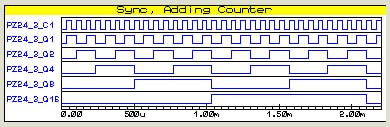
\includegraphics[width=0.90\textwidth]{sync_counter_graph_add.jpg}
    \caption{Графік прямих виходів}
\end{figure}
\begin{figure}[H]
    \centering
    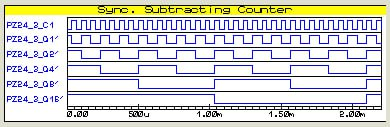
\includegraphics[width=0.90\textwidth]{sync_counter_graph_sub.jpg}
    \caption{Графік непрямих виходів}
\end{figure}
\paragraph{6.}x
\begin{figure}[H]
    \centering
    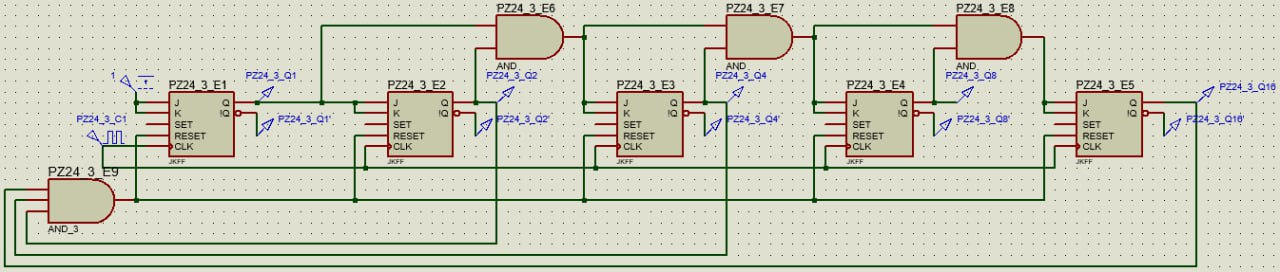
\includegraphics[width=0.90\textwidth]{sync_mod_counter.jpg}
    \caption{Синхронний лічильник по модулю 22}
\end{figure}
\begin{figure}[H]
    \centering
    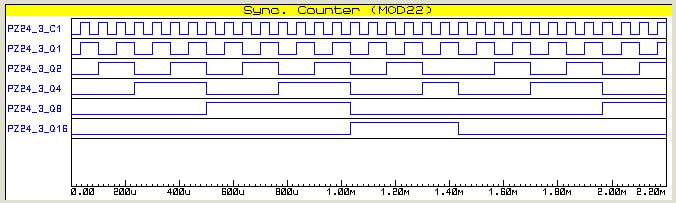
\includegraphics[width=0.90\textwidth]{sync_mod_counter_graph.jpg}
    \caption{Графік}
\end{figure}

\textbf{Висновок:} Я дізнався що таке регістри і лічильники.


\end{document}